\chapter{Data Slicing}

\section*{What is Data Slicing?}

Data slicing is the process of selecting specific parts of a dataset, such as certain rows, columns, or time intervals, for focused analysis. Think of a data set as a large spreadsheet with rows (observations) and columns (variables). Data slicing allows us to extract only the portion we need at the moment. It is a crucial skill in data analysis because it helps us to understand and work with complex data more efficiently.

\section*{Why is Data Slicing Important?}

Data slicing is important for several reasons:
\begin{itemize}
    \item \textbf{Focus on relevant data:} We rarely need the entire dataset at once. Slicing helps us extract just the part we want to study.
    \item \textbf{Improve performance:} Working with smaller subsets reduces memory usage and increases speed, especially for large datasets.
    \item \textbf{Enable deeper insights:} Slicing lets us compare specific groups, such as cities, months, or weather types, within the data set.
    \item \textbf{Prepare for visualization:} Often we only want to visualize a specific variable or a time frame, not the whole dataset.
    \item \textbf{Aid in cleaning and validation:} We can inspect subsets for missing or abnormal values more easily.
\end{itemize}

\section*{Common Types of Slicing}

\begin{itemize}
    \item \textbf{Row Slicing:} Selecting specific observations (e.g., all records for March 2021).
    \item \textbf{Column Slicing:} Selecting specific variables (e.g., only Date and Temperature).
    \item \textbf{Conditional Slicing:} Filtering rows based on conditions (e.g., Temperature > 35 °C).
    \item \textbf{Time-based Slicing:} Extracting data for certain dates or periods.
    \item \textbf{Group-based Slicing:} Filtering data by category (e.g., one district or season).
\end{itemize}

\section*{Examples in R}

\subsection*{Basic Row and Column Slicing}
\begin{verbatim}
# First 10 rows and first 3 columns 
df_climate[1:10, 1:3]
\end{verbatim}

\subsection*{Slicing with Conditions}
\begin{verbatim}
# Days with rainfall greater than 10 mm
df_climate[df_climate$Rainfall > 10, ]
\end{verbatim}

\subsection*{Using \texttt{dplyr} for Readability}
\begin{verbatim}
library(dplyr)
# Days in July with temperature above 32 °C 
df_climate %>% filter(month(Date) == 7, Temperature > 32)
\end{verbatim}

\subsection*{Slicing Time Ranges Using \texttt{tsibble}}
\begin{verbatim}
library(tsibble)
# Data between 2020-06-01 and 2020-08-31 
df_climate %>%
  filter(Date >= as.Date("2020-06-01") & Date <= as.Date("2020-08-31"))
\end{verbatim}

\subsection*{Group-based Slicing}
\begin{verbatim}
# Data for only "Kathmandu" district
df_climate %>%
  filter(District == "Kathmandu")
\end{verbatim}

\section*{Useful Libraries for Data Slicing in R}

\begin{itemize}
    \item \textbf{dplyr} : Offers functions like \texttt{filter()}, \texttt{select()}, \texttt{slice()}, and \texttt{arrange()} for easy row/column selection.
    \item \textbf{tsibble} : Ideal for time series slicing. Lets you work with indexed time data.
    \item \textbf{lubridate} : Helps extract parts of a date (e.g., year, month, weekday) for conditional filtering.
    \item \textbf{data.table} : Very fast slicing, great for large datasets. Syntax is concise and powerful.
\end{itemize}

\section*{Best Practices for Data Slicing}

\begin{itemize}
    \item Use descriptive column names for easier selection.
    \item Always check the structure of your data using \texttt{str()} or \texttt{glimpse()} before slicing.
    \item When slicing by date, ensure the column is in Date format using \texttt{as.Date()}.
    \item Chain multiple operations with \texttt{dplyr} to make slicing more readable.
\end{itemize}

\section{Hilly Region Data Analysis}

The following code filters climate data for selected districts in Nepal’s hilly region and prepares it for a temperature distribution map.

\subsection*{Filtering Districts and Calculating Averages}

\begin{verbatim}
# Create a vector of districts to filter
districts_to_filter <- c("Arghakhanchi","Baglung",
"Baitadi", "Bhaktapur", "Chitwan","Dadeldhura",
"Dailekh", "Dhading", "Dhankuta",  "Dolpa", "Gorkha", 
"Gulmi", "Ilam", "Jumla","Kabhre", "Kaski", 
"Kathmandu", "Lalitpur", "Lamjung", 
"Makwanpur", "Myagdi", 
"Nuwakot", "Okhaldhunga", "Palpa", "Parbat", 
"Rukum", "Salyan", "Sindhuli", "Surkhet",
"Syangja")

# Filter the dataset to only include these districts
filtered_hilly_data <- subset(df_climate, District %in% districts_to_filter)

dim(filtered_hilly_data)
# 413076 25  # example output rows and columns
\end{verbatim}

\subsection*{Geoplot for Temperature Distribution in Hilly Region}

\begin{verbatim}
# Calculate average temperature per district
plot_hilly <- filtered_hilly_data %>%
  group_by(District) %>%
  summarise(
    avg_temp = mean(Temp_2m, na.rm = TRUE),
    avg_precip = mean(Precip, na.rm = TRUE),
    Latitude = first(Latitude),
    Longitude = first(Longitude)
  )

# Merge temperature data with spatial data
nepal_temp_hilly <- left_join(nepal_districts, plot_hilly, by = "District")
\end{verbatim}

% Figure here----------------------------
\begin{figure}[h]
\centering
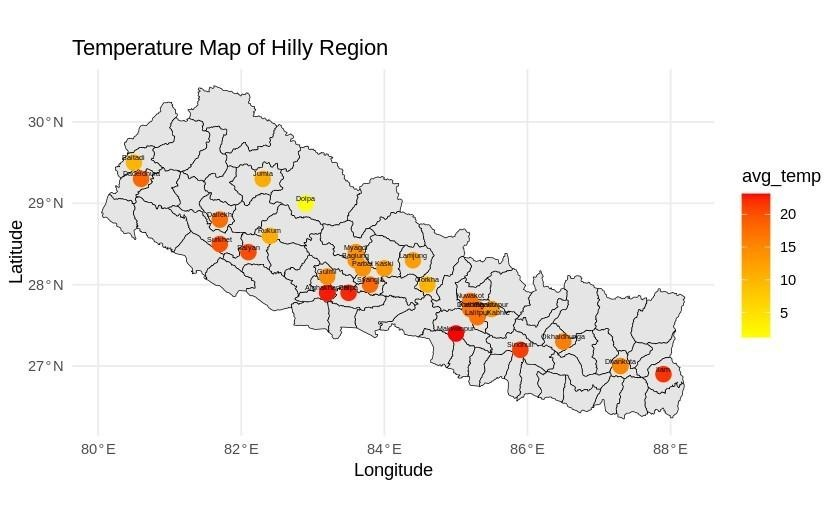
\includegraphics[width=0.6\textwidth]{figures/hilly_map.jpg}
\caption{Temperature Distribution in Nepal using Geoplot
}
\end{figure}

\subsection*{Temperature vs Humidity in the Hilly Region}

The following scatter plot visualizes the relationship between temperature and humidity across districts in the hilly region, colored by season:

\begin{verbatim}
ggplot(filtered_hilly_data, aes(x = Temp_2m, y = Humidity_2m)) +
  geom_point(aes(color = Season), alpha = 0.6) +
  theme_minimal() +
  labs(title = "Temperature vs Humidity in the Hilly Region",
       x = "Temperature (°C)",
       y = "Humidity (%)")
\end{verbatim}

% figure here----------------------------
\begin{figure}[h]
    \centering
    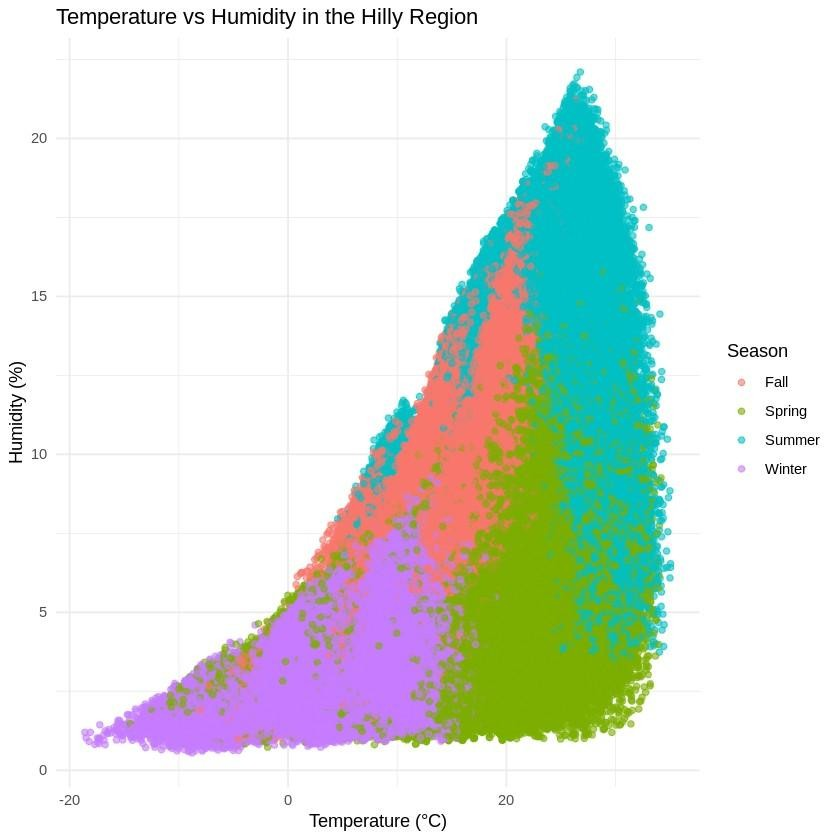
\includegraphics[width=0.5\textwidth]{figures/scatter_hilly.jpg}
    \caption{Scatterplot showing temperature vs humidity according to season}
\end{figure}

\subsubsection*{Insights from Temperature vs Humidity Plot}

\begin{itemize}
    \item A clear positive correlation is observed: higher temperatures generally correspond to higher humidity levels.
    \item Summer shows the highest humidity values, especially above 20\% humidity at moderate to high temperatures.
    \item Winter has the lowest humidity values, often below 10\% even at lower temperatures.
    \item Fall and Spring seasons occupy the middle humidity range, suggesting transitional moisture conditions.
    \item Humidity increases non-linearly with temperature, indicating stronger moisture-holding capacity at warmer temperatures.
    \item A dense clustering of points in summer highlights more consistent humid conditions during that season.
    \item Wider spread of points in winter and spring indicates greater variability in humidity for similar temperature levels.
\end{itemize}

\subsection*{Average Precipitation by District}

\begin{verbatim}
avg_precip_by_district <- filtered_hilly_data %>%
  group_by(District) %>%
  summarise(avg_precip = mean(Precip, na.rm = TRUE))

ggplot(avg_precip_by_district, aes(x = reorder(District, -avg_precip),
 y = avg_precip)) +
  geom_bar(stat = "identity", fill = "skyblue") +
  theme_minimal() +
  labs(title = "Average Precipitation by District",
       x = "District", y = "Average Precipitation") +
  theme(axis.text.x = element_text(angle = 90, hjust = 1))
\end{verbatim}

% Figure here----------------------------
\begin{figure}[h]
    \centering
    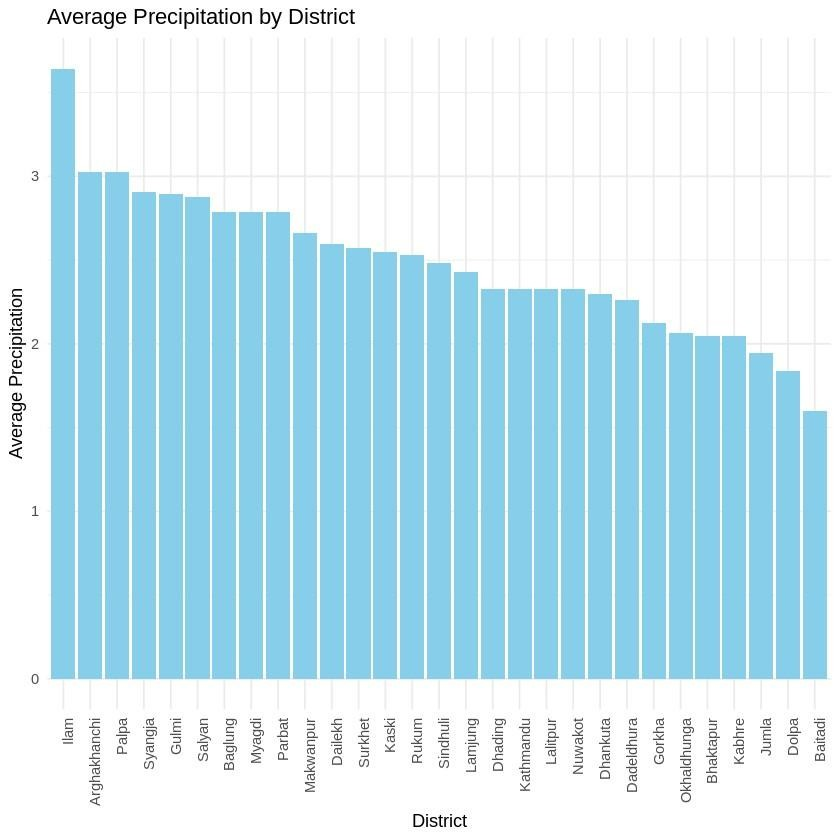
\includegraphics[width=0.5\textwidth]{figures/bar_hilly.jpg}
    \caption{Bar Chart of Average Precipitation in Hilly Region Districts}
\end{figure}

\subsection*{Boxplot of Seasonal Precipitation in Hilly Districts}

\begin{verbatim}
ggplot(filtered_hilly_data, aes(x = Season, y = Precip, fill = Season)) +
  geom_boxplot() +
  labs(title = "Seasonal Precipitation in Hilly Districts",
       x = "Season", y = "Precipitation (mm)") +
  theme_minimal()
\end{verbatim}

% Figure here-----------------------------
\begin{figure}[h]
    \centering
    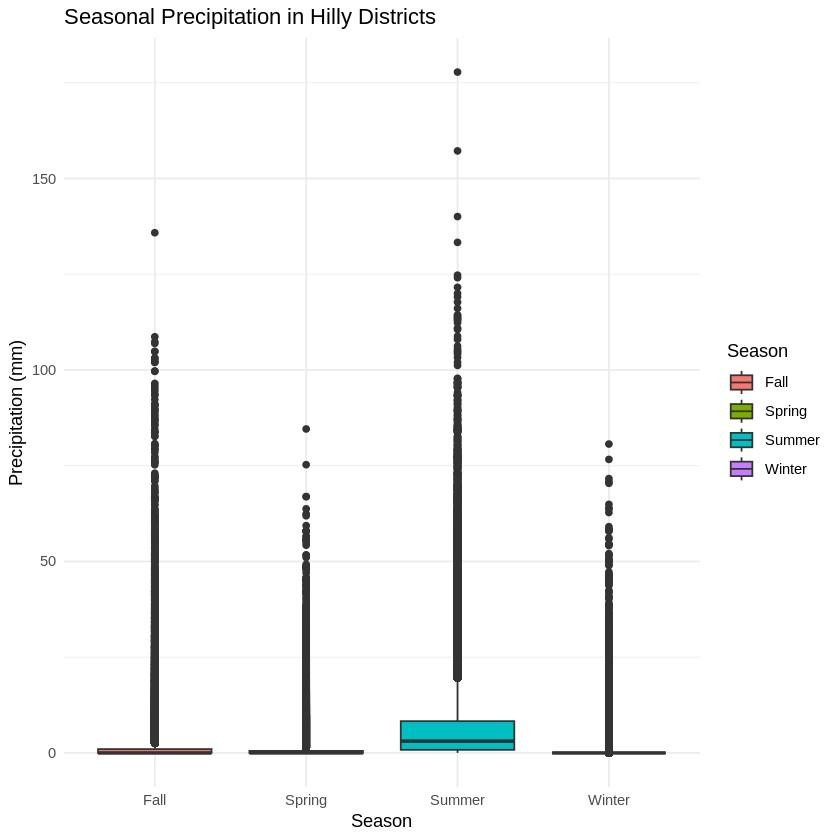
\includegraphics[width=0.5\textwidth]{figures/box_hilly.jpg}
    \caption{Seasonal Precipitation Distribution in Hilly Districts}
\end{figure}

\subsubsection*{Insights from Seasonal Precipitation Plot}

\begin{itemize}
    \item Summer records the highest median and variability in precipitation, indicating it as the peak rainy season.
    \item Spring, Fall, and Winter show comparatively lower median precipitation, clustered near zero.
    \item Despite low medians, all seasons exhibit outliers with precipitation events exceeding 100 mm.
    \item The box for Summer is significantly taller, suggesting a broader interquartile range and more frequent moderate to heavy rainfalls.
    \item Fall and Winter have tight boxes with few extreme outliers, indicating rare but intense rain events.
    \item Spring shows almost no visible box, suggesting highly concentrated low precipitation with sporadic extremes.
    \item Overall, precipitation in hilly districts is highly seasonal, with summer dominating rainfall contributions.
\end{itemize}

\subsection*{Density Plot of Relative Humidity Across Hilly Districts}

\begin{verbatim}
ggplot(filtered_hilly_data, aes(x = RH_2m, fill = District)) +
  geom_density(alpha = 0.4) +
  labs(title = "Humidity Distribution Across Hilly Districts",
       x = "Relative Humidity (%)", y = "Density") +
  theme_minimal()
\end{verbatim}

\begin{figure}[h]
    \centering
    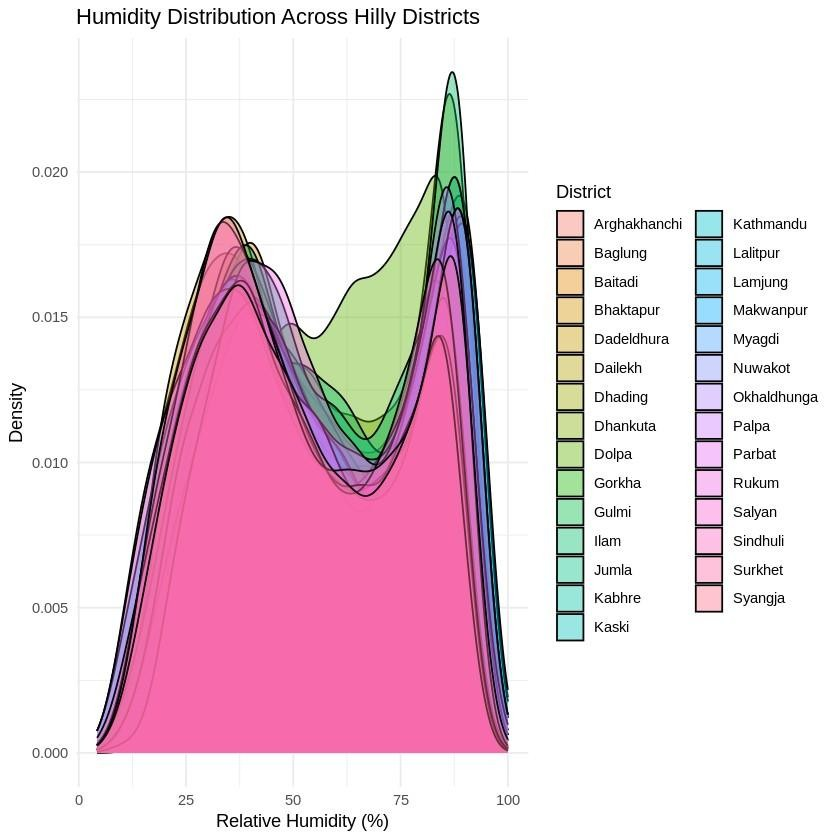
\includegraphics[width=0.5\textwidth]{figures/humid_hilly.jpg}
    \caption{Humidity Distribution Across Hilly Districts}
\end{figure}

\subsubsection*{Insights from Humidity Distribution}

\begin{itemize}
    \item The distribution is bimodal, indicating distinct dry and wet seasonal patterns.
    \item High relative humidity levels (75–90\%) are common across many districts.
    \item Districts like Rukum show broader density curves, suggesting higher variability in humidity.
    \item Districts such as Kathmandu and Dhankuta have sharper peaks, indicating more stable humidity conditions.
    \item Overlapping curves among districts point to similar climatic conditions in the hilly region.
    \item Tails extending towards 0\% and 100\% imply the occurrence of rare extreme humidity events.
    \item These patterns help identify humidity-prone areas useful for agricultural and climatic planning.
\end{itemize}

\subsection*{Extreme Precipitation Analysis in Hilly Regions}

Understanding extreme rainfall events is crucial for disaster preparedness, especially in hilly terrains where intense precipitation can trigger flash floods and landslides. This section presents an analysis of high-impact rainfall events in such regions based on the 95th percentile threshold.

\subsubsection*{Monthly Precipitation Trends}

We begin by computing average monthly precipitation for each year to examine seasonal variation.

\begin{verbatim}
monthly_precip_hilly <- filtered_hilly_data %>%
  group_by(Month_Number, Year = as.numeric(format(Date, "%Y"))) %>%
  summarize(Avg_Precip = mean(Precip, na.rm = TRUE))
\end{verbatim}

\subsubsection*{Defining Extreme Rainfall Events}

To isolate extreme rainfall events, we compute the 95th percentile of all precipitation values. Events exceeding this threshold are classified as extreme.

\begin{verbatim}
# Calculate the 95th percentile of Precipitation
extreme_threshold <- quantile(filtered_hilly_data$Precip, 0.95, na.rm = TRUE)

# Filter the extreme events
extreme_events_hilly <- filtered_hilly_data %>%
filter(Precip > extreme_threshold)

print(extreme_threshold)

95%
13.51
\end{verbatim}

\subsubsection*{Yearly Trend of Extreme Events}

We extract the year from each event and calculate the yearly frequency of extremes to visualize how often such events occur over time.

\begin{verbatim}
# Extract year and count extreme events per year
extreme_events_hilly$Year <- format(extreme_events_hilly$Date, "%Y")
yearly_extreme <- extreme_events_hilly %>%
group_by(Year) %>%
  summarize(Count = n())

# Plot yearly frequency
ggplot(yearly_extreme, aes(x = as.numeric(Year), y = Count)) +
geom_line() +
geom_point() +
labs(
  title = "Yearly Frequency of Extreme Precipitation Events",
  x = "Year",
  y = "Number of Extreme Events")
\end{verbatim}

% Figure here-----------------------------
\begin{figure}[h]
    \centering
    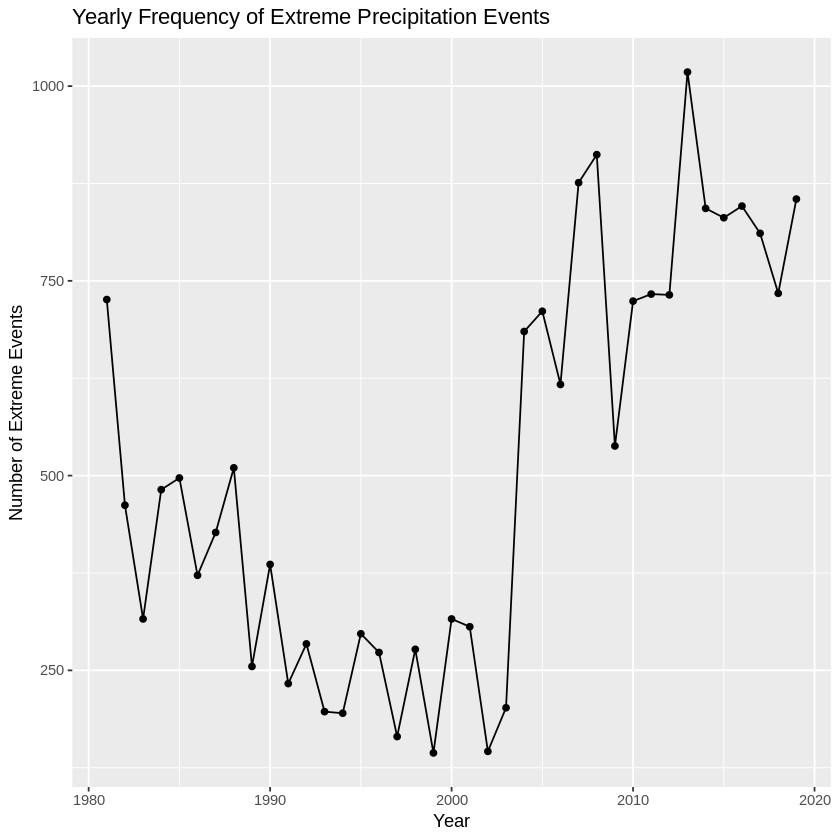
\includegraphics[width=0.5\textwidth]{figures/trend_hilly.jpg}
    \caption{Yearly Frequency of Extreme Precipitation Events}
\end{figure}

\subsubsection*{Yearly Trends}

\begin{itemize}
    \item Low and fluctuating frequency of extreme events from 1980 to early 2000s.
    \item Sharp increase in events post-2003, with a peak around 2013.
    \item Suggests rising climate variability and increased flood risk in recent decades.
\end{itemize}

\subsubsection*{Monthly Distribution of Extreme Events}

To identify seasonal flood risk, we count the number of extreme events in each month and visualize the distribution.

\begin{verbatim}
# Count extreme events per month
monthly_extremes <- extreme_events_hilly %>%
group_by(Month_Label) %>%
  summarize(Count = n())

# Plot the counts
ggplot(monthly_extremes, aes(x = Month_Label, y = Count)) +
geom_bar(stat = "identity", fill = "red") +
labs(
  title = "Number of Extreme Events Per Month",
  x = "Month", 
  y = "Count of Extreme Events")
\end{verbatim}

% Figure here-----------------------------
\begin{figure}[h]
    \centering
    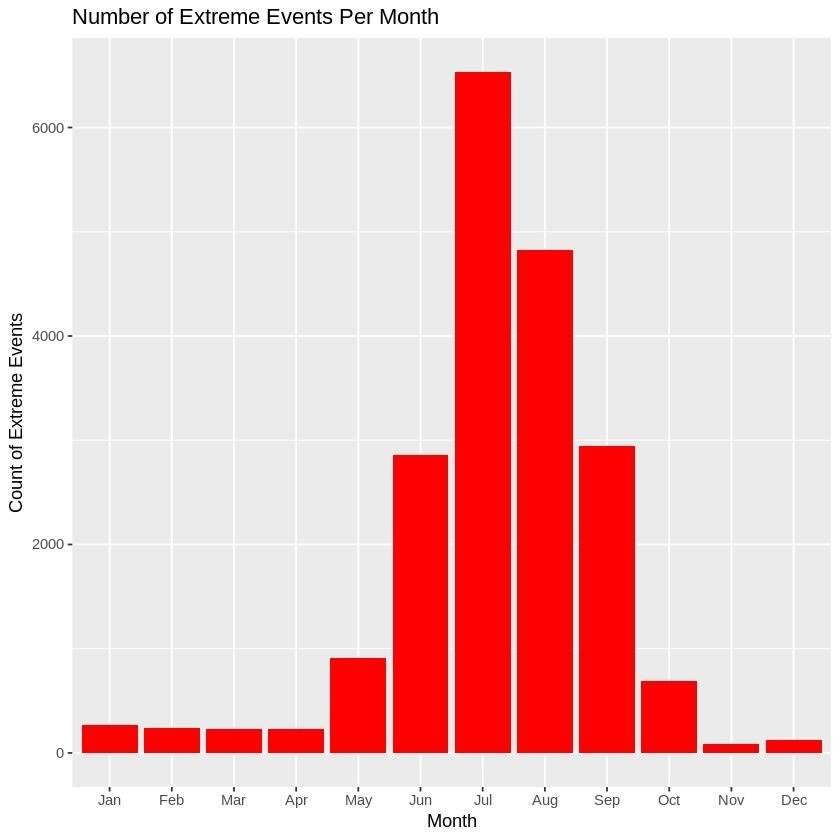
\includegraphics[width=0.5\textwidth]{figures/extreme_hilly.jpg}
    \caption{Number of Extreme Precipitation Events Per Month}
\end{figure}

\subsubsection*{Monthly Patterns}

\begin{itemize}
    \item Highest number of extreme events observed in July, followed by August and June.
    \item May and September show moderate activity—transitional monsoon months.
    \item Winter and spring months (November–April) show minimal extreme events.
\end{itemize}

\section*{Conclusion}

The analysis clearly highlights both a temporal increase in extreme rainfall events over the years and a strong seasonal concentration during the monsoon months. These findings emphasize the need for targeted flood preparation strategies, especially from June to September, and call for continuous monitoring and adaptation planning to improve climate resilience in vulnerable regions.


\section{Western Region Climate Data Analysis}

This analysis shows the temperature distribution across districts in the Western region of Nepal using spatial data visualization.

\subsection*{Filtering Districts}

\begin{verbatim}
# List of districts to match
district_list <- c("Gorkha", "Kaski", "Lamjung", "Manang", "Syangja",
                   "Arghakhanchi", "Gulmi",
                   "Nawalparasi", "Palpa", "Rupandehi", "Baglung",
                   "Myagdi", "Parbat","Mustang")

filtered_data_western <- df_climate[df_climate$District%in% district_list,]
\end{verbatim}

\subsection*{Geoplot for Temperature Distribution in Western Region}

\begin{verbatim}
# Calculate average temperature per district
plot_western <- filtered_data_western %>%
  group_by(District) %>%
  summarise(
    avg_temp = mean(Temp_2m, na.rm = TRUE),
    Latitude = first(Latitude),
    Longitude = first(Longitude)
  )

# Merge temperature data with spatial data
nepal_temp_west <- left_join(nepal_districts, plot_western , by = "District")

# GeoplotPlot
ggplot(data = nepal_temp_west) +
geom_sf(aes(data = avg_temp), color = "black") +
geom_point(aes(x = Longitude, y = Latitude, color = avg_temp), 
  size = 4) +  # Points for avg_temp
geom_text(data = plot_western, aes(
  x = Longitude, 
  y = Latitude, 
  label = District),
  size = 1.5, vjust = -0.5, color = "black") +
scale_color_gradient(low = "yellow", high = "red") +  # Color scale
labs(
  title = "Temperature Map of Nepal", fill = "Temperature"
  ) +
theme_minimal()
\end{verbatim}

% Figure here-----------------------------
\begin{figure}[h]
    \centering
    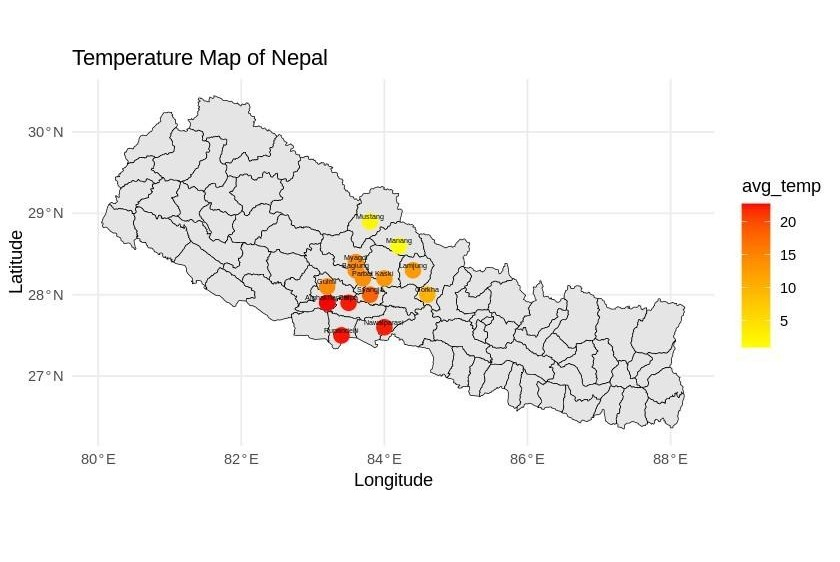
\includegraphics[width=0.6\textwidth]{figures/map_west.jpg}
    \caption{Temperature Map of Western Region}
\end{figure}

\subsection*{Scatter Plot of Temperature vs. Precipitation with Wind Speed by Season}

\begin{verbatim}
ggplot(filtered_data_western, aes(
  x = Temp_2m, 
  y = Precip, 
  color = Season, 
  size = WindSpeed_10m)) +
geom_point(alpha = 0.7) +
scale_color_manual(values = c(
    "Spring" = adjustcolor("yellow", alpha.f = 0.6),
    "Summer" = adjustcolor("red", alpha.f = 0.6),
    "Fall" = adjustcolor("orange", alpha.f = 0.6),
    "Winter" = adjustcolor("blue", alpha.f = 0.6)
  )) +
scale_size_continuous(range = c(1, 10)) +
labs(
title = "Scatter Plot of Temperature vs. Precipitation with Wind Speed Size",
x = "Temperature (°C)",
y = "Precipitation (mm/day)",
color = "Season",
size = "Wind Speed (10m)"
) +

theme_minimal()
\end{verbatim}

% Figure here-----------------------------
\begin{figure}[h]
    \centering
    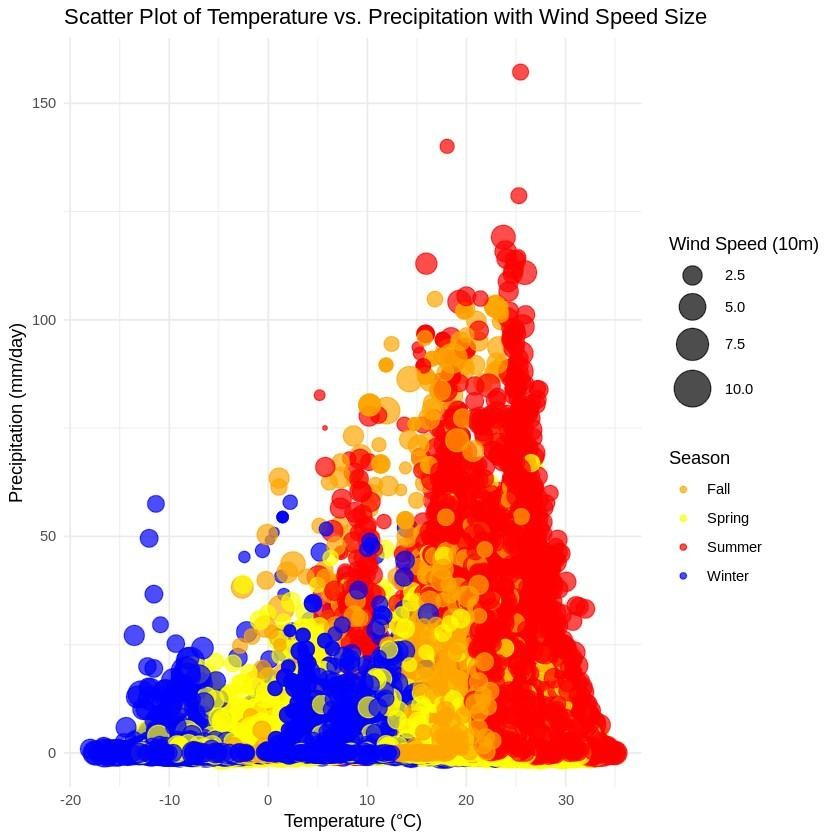
\includegraphics[width=0.5\textwidth]{figures/scatter_west.jpg}
    \caption{Scatterplot showing Temperature vs. Precipitation with Wind Speed by Season}
    \label{fig:scatter_temp_precip_wind}
\end{figure}

\subsection*{Histogram of Wind Speed with Density Curve for Western Region}

\begin{verbatim}
ggplot(filtered_data_western, aes(x = WindSpeed_10m)) +
geom_histogram(aes(y = ..density..), bins = 30, fill = "skyblue", 
color = "black", alpha = 0.7) + 
geom_density(color = "blue", linewidth = 1) + 
labs(
title = "Histogram of Wind Speed with Density Trendline for Western Region",
x = "Wind Speed (10m)",
y = "Density") +
theme_minimal()
\end{verbatim}

% Figure here-----------------------------
\begin{figure}[h]
    \centering
    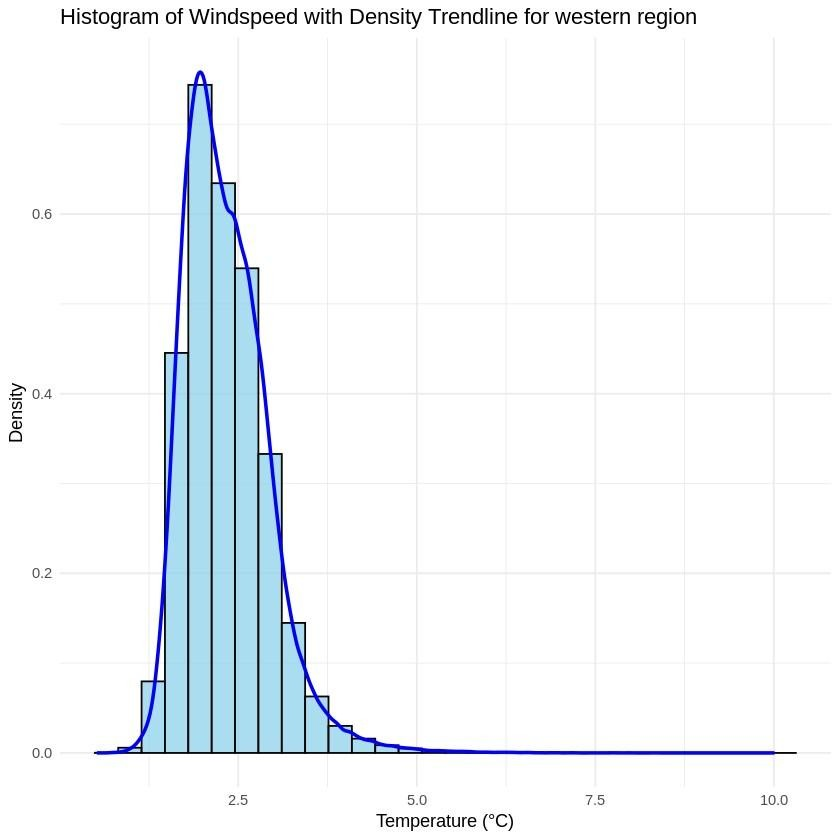
\includegraphics[width=0.5\textwidth]{figures/hist_west.jpg}
    \caption{Histogram of Wind Speed with Density Trendline for Western Region}
\end{figure}

\subsection*{Precipitation Trend Over Time in Western Region}

\begin{verbatim}
ggplot(filtered_data_western, 
aes(
  x = Date, 
  y = Precip)) +
geom_line(color = "blue") +
labs(
  title = "Precipitation Trend Over Time - Western Region",
  x = "Date", 
  y = "Precipitation (mm)") +

  theme_minimal()
\end{verbatim}

% Figure here--------------------------
\begin{figure}[h]
    \centering
    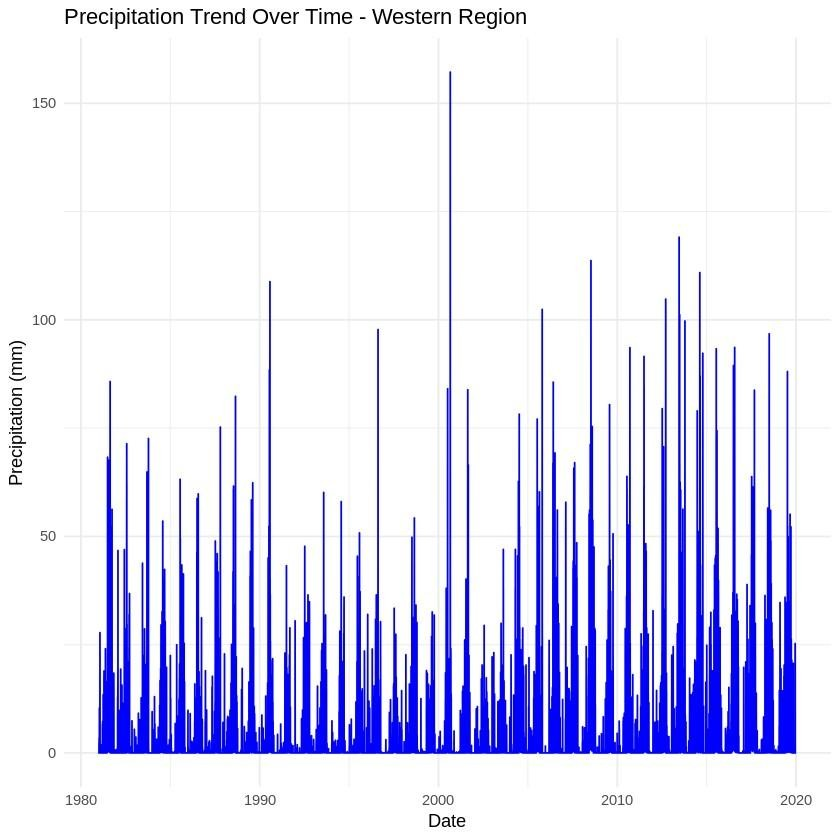
\includegraphics[width=0.5\textwidth]{figures/precip_west.jpg}
    \caption{Precipitation Trend Over Time - Western Region}
\end{figure}

\subsection*{Temperature Distribution by Season}

\begin{verbatim}
ggplot(filtered_data_western, aes(x = Season, y = Temp_2m, fill = Season)) +
  geom_boxplot() +
  labs(title = "Temperature Distribution by Season",
       x = "Season", y = "Temperature (°C)") +
  theme_minimal() +
  theme(legend.position = "none")
\end{verbatim}

% Figure here-----------------------------
\begin{figure}[h]
    \centering
    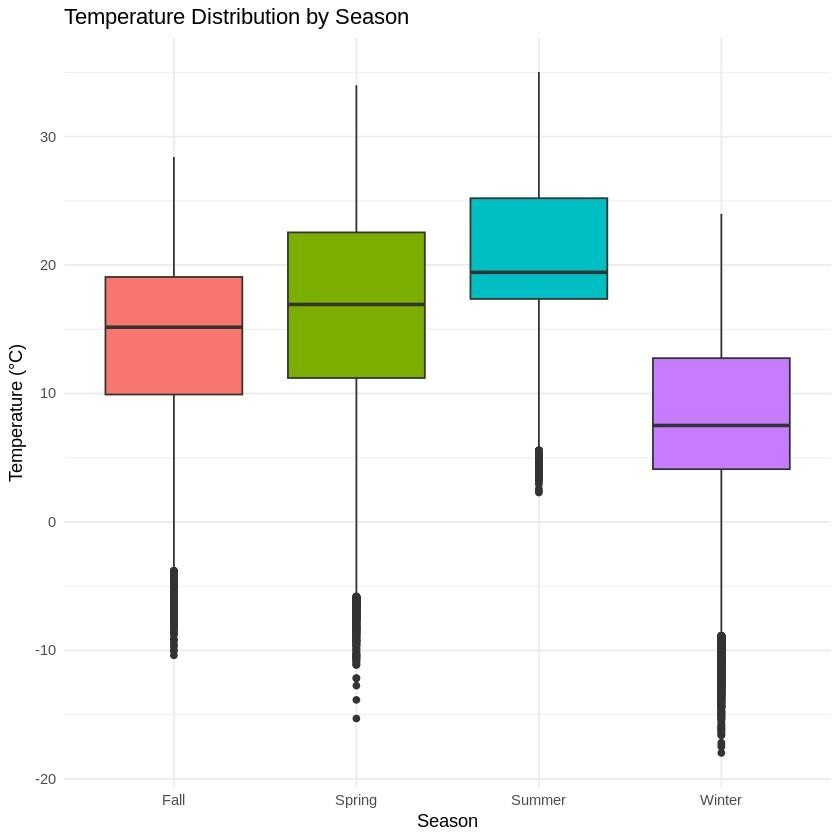
\includegraphics[width=0.5\textwidth]{figures/box_west.jpg}
    \caption{Temperature Distribution by Season in Western Region}
\end{figure}

\section{Time Based Data Analysis (May - August)}

This section filters data for the seasonal months of May through August and visualizes various climate variables including precipitation, humidity, temperature, wind speed, and their distributions.

\subsection*{Filtering Seasonal Months}

\begin{verbatim}
time_based_filter <- df_climate %>%
   dplyr::filter(Month_Label %in% c("May","Jun","Jul","Aug"))
dim(time_based_filter)
\end{verbatim}

\subsection*{Comparison of Precipitation and Humidity by Month}

\begin{verbatim}
precip_temp_data_long <- pivot_longer(precip_temp_data, 
cols = c(Avg_Precip, Avg_humid), 
names_to = "Variable", values_to = "Value")

ggplot(precip_temp_data_long, aes(x = Month_Label, y = Value, 
fill = Variable)) +
geom_bar(stat = "identity", position = "dodge") +
labs(
  title = "Comparison of Precipitation and Humidity by Month",     
  x = "Month", 
  y = "Value") +
  theme_minimal()
\end{verbatim}

% Figure here--------------------
\begin{figure}[h]
    \centering
    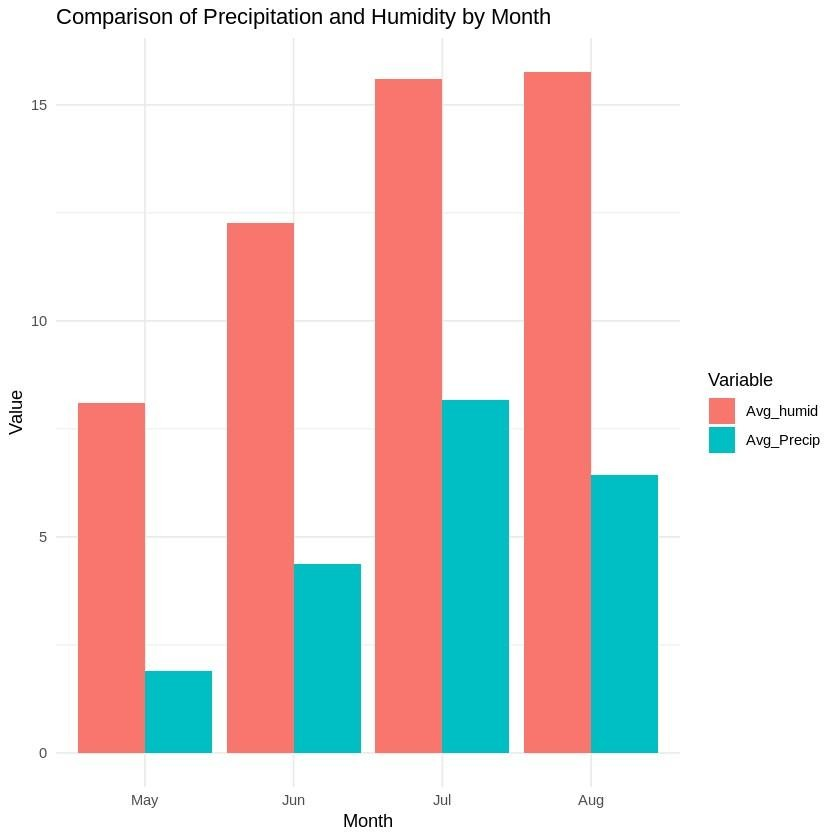
\includegraphics[width=0.5\textwidth]{figures/bar_time.jpg}
    \caption{Bar chart showing precipitation and humidity by month (May to August)}
\end{figure}

\subsection*{Relative Humidity vs Temperature for May to August}

\begin{verbatim}
ggplot(time_based_filter, aes(
  x = Temp_2m, 
  y = RH_2m)) +
geom_point(alpha = 0.3, color = "blue") +
labs(
    title = "Relative Humidity vs Temperature (May - Aug)",
    x = "Temperature (°C)", 
    y = "Relative Humidity (%)") +
  
theme_minimal()
\end{verbatim}

% Figure here-----------------------------
\begin{figure}[h]
    \centering
    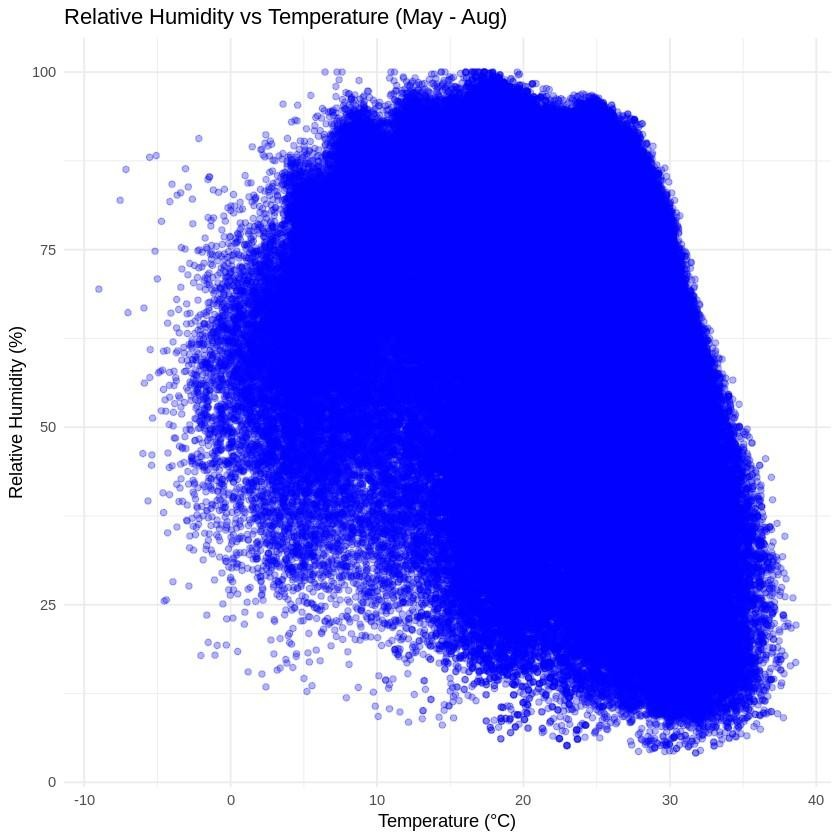
\includegraphics[width=0.5\textwidth]{figures/scatter_time.jpg}
    \caption{Scatterplot showing Temperature vs Relative Humidity (May to August)}
\end{figure}

\subsection*{Wind Speed Range at 10m by Month}

\begin{verbatim}
ggplot(time_based_filter, aes(
  x = Month_Label, 
  y = WindSpeedRange_10m, 
  fill = Month_Label)) +
geom_boxplot() +
labs(
  title = "Wind Speed Range at 10m by Month",
  x = "Month", 
  y = "Wind Speed Range (m/s)") +
  theme_minimal() +
  theme(legend.position = "none")
\end{verbatim}

\begin{figure}[h]
    \centering
    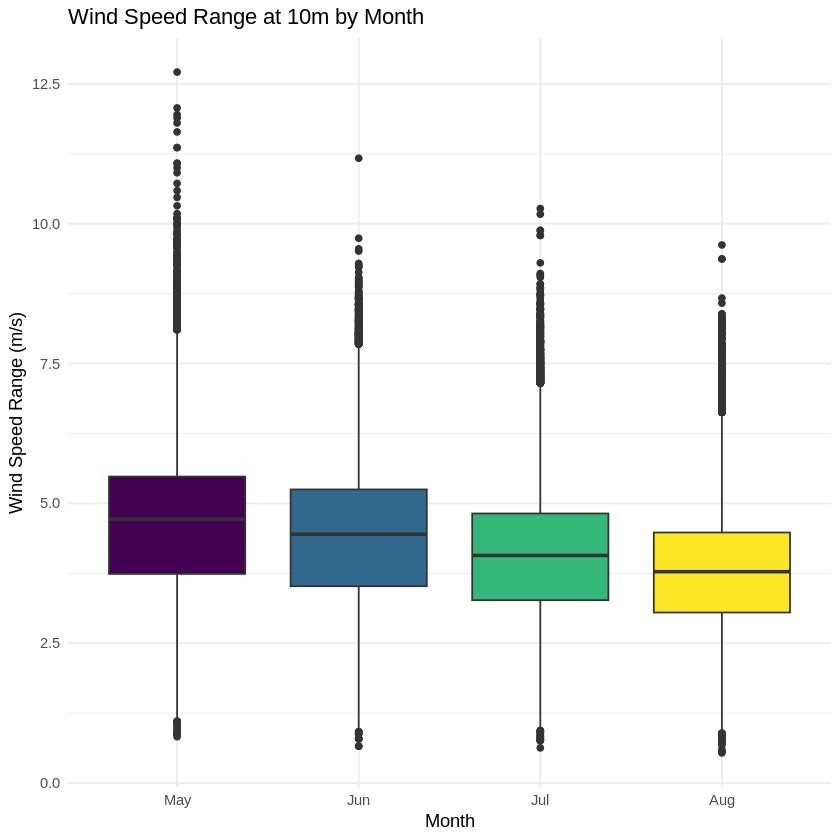
\includegraphics[width=0.5\textwidth]{figures/box_time.jpg}
    \caption{Boxplot of Wind Speed Range at 10m by Month (May to August)}
\end{figure}

\subsection*{Average Temperature Heatmap by District and Month}

To find out how temperature varies by district across different months, we created a heatmap that shows the average temperature for each district by month. This visualization helps us quickly identify seasonal patterns and regional differences in temperature across Nepal.
\begin{verbatim}
library(reshape2)

avg_temp_district <- time_based_filter %>%
  group_by(District, Month_Label) %>%
  summarise(
    AvgTemp = mean(Temp_2m, na.rm = TRUE)) %>%
  ungroup()

ggplot(avg_temp_district, aes(
  x = Month_Label, 
  y = District, 
  fill = AvgTemp)) +
  geom_tile() +
  scale_fill_viridis_c(option = "plasma") +
  labs(
    title = "Average Temperature by District and Month",
    x = "Month", 
    y = "District", 
    fill = "Avg Temp (°C)") +

  theme_minimal() +

  theme(axis.text.y = element_text(size = 6))
\end{verbatim}

% Figure here-----------------------------
\begin{figure}[h]
    \centering
    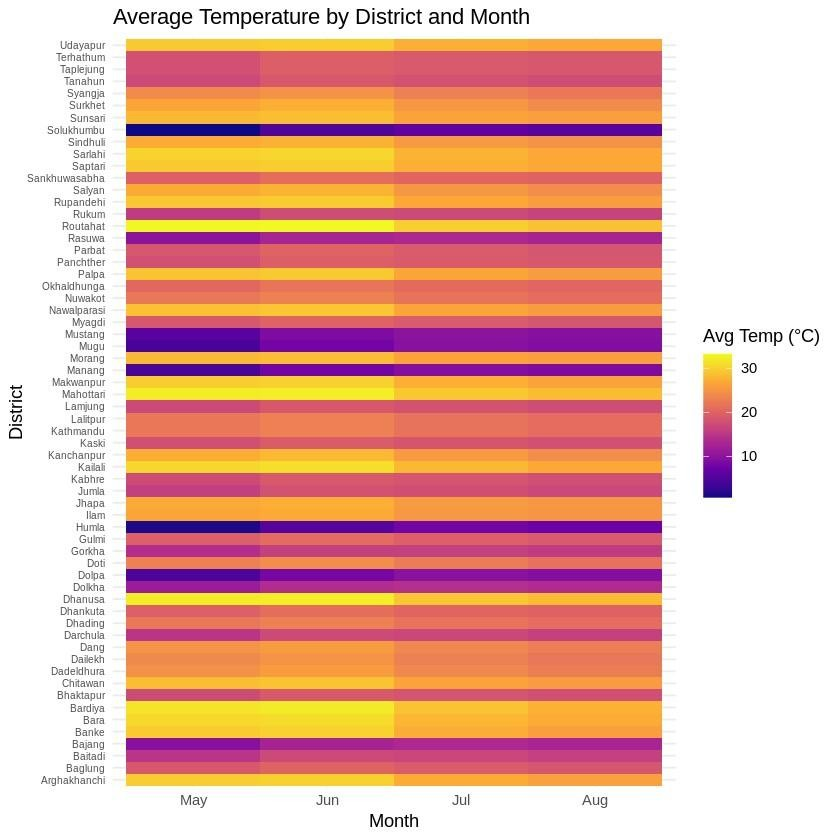
\includegraphics[width=0.6\textwidth]{figures/heatmap_time.jpg}
    \caption{Average Temperature Heatmap by District and Month (May to August)}
    \label{fig:avg_temp_heatmap}
\end{figure}

\subsection*{Density Plot of Temperature by Month}

\begin{verbatim}
ggplot(time_based_filter, aes(x = Temp_2m, fill = Month_Label)) +
  geom_density(alpha = 0.5) +
  labs(title = "Temperature Density by Month (May-August)",
       x = "Temperature (°C)", y = "Density") +
  theme_minimal()
\end{verbatim}

% Figure here------------------------
\begin{figure}[h]
    \centering
    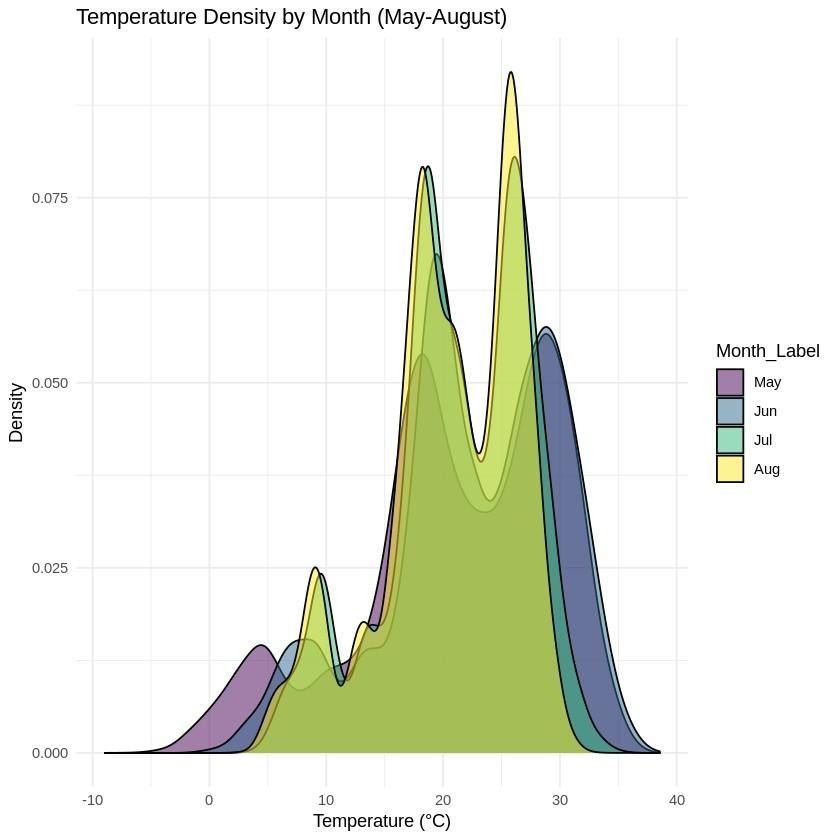
\includegraphics[width=0.45\textwidth]{figures/density_time.jpg}
    \caption{Density plot of Temperature distribution by month (May to August)}
    \label{fig:temp_density}
\end{figure}
